\documentclass[tikz,border=10pt]{standalone}

% Essential packages for TikZ
\usepackage{tikz}
\usepackage{graphicx}
\usepackage{amsmath}
\usepackage{calc}

% Additional TikZ libraries that might be needed
\usetikzlibrary{positioning,calc,arrows.meta}

% Define the \scalebox command if not using the graphicx package already
\usepackage{graphics}

% Figure size
\newlength\figureheight
\newlength\figurewidth
\newlength{\imspacing}

% Latin
\newcommand{\eg}{\textit{e.g.}}
\newcommand{\ie}{\textit{i.e.}}
\newcommand{\cf}{\textit{cf.}}
\newcommand{\etc}{\textit{etc.}}
\newcommand{\etal}{\textit{et~al.}}

% Math
\newcommand{\mathbold}[1]{\bm{#1}}
\newcommand{\mbf}[1]{\mathbf{#1}}
\newcommand{\vect}[1]{\mathbf{#1}}
\newcommand{\vectb}[1]{\bm{#1}}
\newcommand{\T}{^\mathsf{T}}
\newcommand{\mat}[1]{\mathbf{#1}}
\newcommand{\kron}{\raisebox{1pt}{\ensuremath{\:\otimes\:}}} % Kronceker product
\newcommand{\bigO}{\mathcal{O}}

% Custom macros
%\newcommand{\T}{\top}    % Transpose
\newcommand{\dd}{\,\mathrm{d}} % E.g. \int f(x) \dd x
\newcommand{\E}{\mathbb{E}}    % Expectation
\newcommand{\R}{\mathbb{R}}    % Real numbers
\newcommand{\N}{\mathrm{N}}   % Gaussian distribution
\DeclareMathOperator{\tr}{tr}
\DeclareMathOperator{\diag}{diag}
\DeclareMathOperator{\chol}{chol}
\DeclareMathOperator{\dchol}{dchol}
\DeclareMathOperator{\Cov}{Cov}
\DeclareMathOperator{\Var}{Var}
\DeclareMathOperator{\gammad}{Gamma}
\DeclareMathOperator{\expd}{Exp}
\DeclareMathOperator{\sech}{sech}
%\DeclareMathOperator{\U}{U}
\DeclareMathOperator{\argmin}{arg\,min}
\DeclareMathOperator{\argmax}{arg\,max}
\newcommand{\KL}[2]{\mathrm{D}_\mathrm{KL}\left[#1\|#2\right]}

% Bold Greek symbols
\newcommand{\valpha}[0]{\mathbold{\alpha}}
\newcommand{\vbeta}[0]{\mathbold{\beta}}
\newcommand{\vsigma}[0]{\mathbold{\sigma}}
\newcommand{\vchi}[0]{\mathbold{\chi}}
\newcommand{\vepsilon}[0]{\mathbold{\varepsilon}}
\newcommand{\veta}[0]{\mathbold{\eta}}
\newcommand{\vmu}[0]{\mathbold{\mu}}
\newcommand{\vomega}[0]{\mathbold{\omega}}
\newcommand{\vxi}[0]{\mathbold{\xi}}
\newcommand{\vphi}[0]{\mathbold{\phi}}
\newcommand{\vtheta}[0]{\mathbold{\theta}}
\newcommand{\vTheta}[0]{\mathbold{\Theta}}
\newcommand{\vzeta}[0]{\mathbold{\zeta}}
\newcommand{\MPsi}[0]{\mathbold{\Psi}}
\newcommand{\MPhi}[0]{\mathbold{\Phi}}
\newcommand{\MSigma}[0]{\mathbold{\Sigma}}
\newcommand{\MTheta}[0]{\mathbold{\Theta}}
\newcommand{\invchisq}[0]{\mathrm{Inv\text{-}}\chi^2}
\renewcommand{\mid}{\,|\,}
\newcommand{\imag}[0]{\mathrm{i}}
\def\x{\mathbf{x}}
\def\y{\mathbf{y}}
\def\G{\mathbf{G}}
\def\Q{\mathbf{Q}}
\def\R{\mathbf{R}}
\def\bR{\mathbb{R}}
\def\e{\mathbf{e}}
\def\X{\mathbf{X}}
\def\H{\mathbf{H}}
\def\h{\mathbf{h}}
\def\Y{\mathbf{Y}}
\def\E{\mathbf{E}}
\def\P{\mathbf{P}}
\def\p{\mathbf{p}}
\def\N{\mathcal{N}}
\def\U{\mathbf{U}}
\def\enc{\boldsymbol{\varphi}}

% Use these macros for big roman symbols
\newcommand{\RL}{\mathrm{L}}
\newcommand{\RM}{\mathrm{M}}
\newcommand{\RQ}{\mathrm{Q}}
\newcommand{\RS}{\mathrm{S}}
\newcommand{\RU}{\mathrm{U}}

% Use these macros for roman symbols
\newcommand{\rb}{\mathrm{b}}
\newcommand{\rc}{\mathrm{c}}
\newcommand{\rrm}{\mathrm{m}}
\newcommand{\ro}{\mathrm{o}}
\newcommand{\rs}{\mathrm{s}}
\newcommand{\rrq}{\mathrm{q}}

% Use these macros for vectors and matrices
\newcommand{\va}{\mbf{a}}
\newcommand{\vb}{\mbf{b}}
\newcommand{\vc}{\mbf{c}}
\newcommand{\vd}{\mbf{d}}
\newcommand{\ve}{\mbf{e}}
\newcommand{\vf}{\mbf{f}}
\newcommand{\vg}{\mbf{g}}
\newcommand{\vh}{\mbf{h}}
\newcommand{\vi}{\mbf{i}}
\newcommand{\vj}{\mbf{j}}
\newcommand{\vk}{\mbf{k}}
\newcommand{\vl}{\mbf{l}}
\newcommand{\vm}{\mbf{m}}
\newcommand{\vn}{\mbf{n}}
\newcommand{\vo}{\mbf{o}}
\newcommand{\vp}{\mbf{p}}
\newcommand{\vq}{\mbf{q}}
\newcommand{\vr}{\mbf{r}}
\newcommand{\vs}{\mbf{s}}
\newcommand{\vu}{\mbf{u}}
\newcommand{\vv}{\mbf{v}}
\newcommand{\vw}{\mbf{w}}
\newcommand{\vx}{\mbf{x}}
\newcommand{\vy}{\mbf{y}}
\newcommand{\vz}{\mbf{z}}
\newcommand{\MA}{\mbf{A}}
\newcommand{\MB}{\mbf{B}}
\newcommand{\MC}{\mbf{C}}
\newcommand{\MD}{\mbf{D}}
\newcommand{\MF}{\mbf{F}}
\newcommand{\MG}{\mbf{G}}
\newcommand{\MH}{\mbf{H}}
\newcommand{\MI}{\mbf{I}}
\newcommand{\MJ}{\mbf{J}}
\newcommand{\MK}{\mbf{K}}
\newcommand{\ML}{\mbf{L}}
\newcommand{\MM}{\mbf{M}}
\newcommand{\MP}{\mbf{P}}
\newcommand{\MQ}{\mbf{Q}}
\newcommand{\MR}{\mbf{R}}
\newcommand{\MS}{\mbf{S}}
\newcommand{\MT}{\mbf{T}}
\newcommand{\MV}{\mbf{V}}
\newcommand{\MW}{\mbf{W}}
\newcommand{\MX}{\mbf{X}}
\newcommand{\MY}{\mbf{Y}}


% Random matrices
\def\mA{{\bm{A}}}
\def\mB{{\bm{B}}}
\def\mC{{\bm{C}}}
\def\mD{{\bm{D}}}
\def\mE{{\bm{E}}}
\def\mF{{\bm{F}}}
\def\mG{{\bm{G}}}
\def\mH{{\bm{H}}}
\def\mI{{\bm{I}}}
\def\mJ{{\bm{J}}}
\def\mK{{\bm{K}}}
\def\mL{{\bm{L}}}
\def\mM{{\bm{M}}}
\def\mN{{\bm{N}}}
\def\mO{{\bm{O}}}
\def\mP{{\bm{P}}}
\def\mQ{{\bm{Q}}}
\def\mR{{\bm{R}}}
\def\mS{{\bm{S}}}
\def\mT{{\bm{T}}}
\def\mU{{\bm{U}}}
\def\mV{{\bm{V}}}
\def\mW{{\bm{W}}}
\def\mX{{\bm{X}}}
\def\mY{{\bm{Y}}}
\def\mZ{{\bm{Z}}}

% Document begins
\begin{document}

\begin{tikzpicture}
% Styles
%\tikzstyle{label}=[font=\tiny]
\tikzstyle{arr}=[->,-latex,line width=1pt]
% The left image (reactants) - moved further left
\node[anchor=center,inner sep=0] (image) at (-20,0){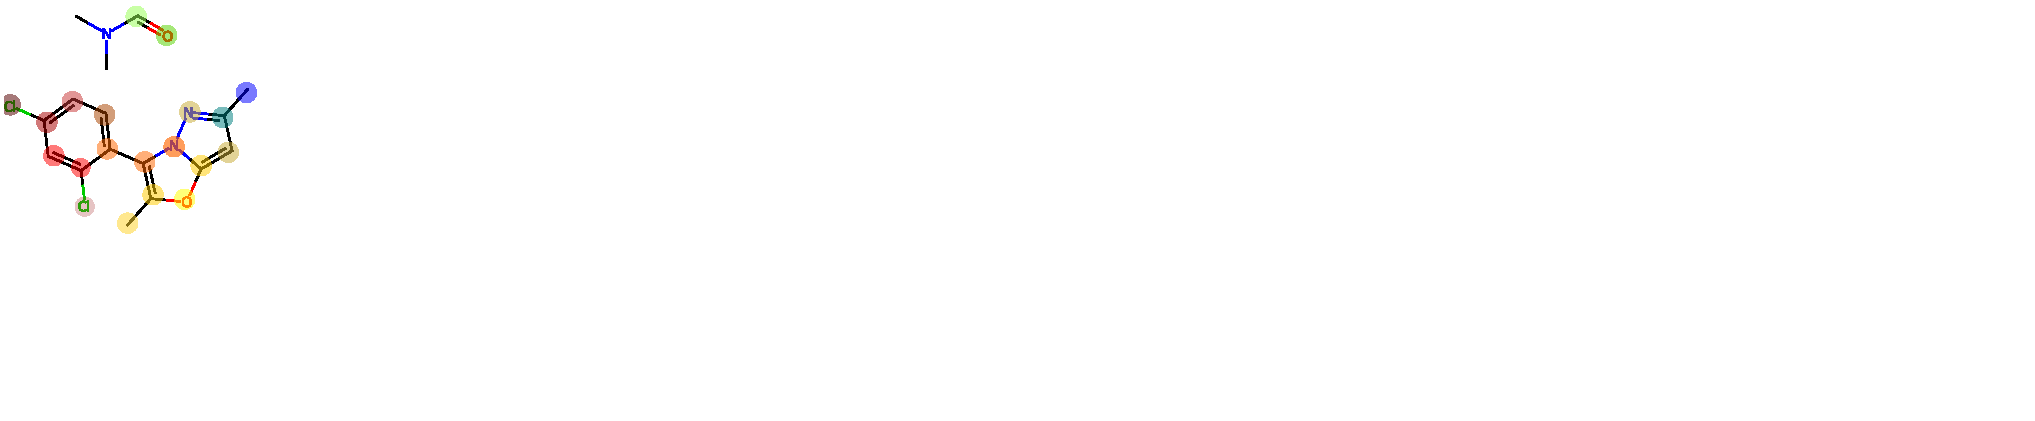
\includegraphics[width=10cm,height=6cm,keepaspectratio]{fig/reactants.pdf}};
\node[anchor=center,inner sep=0](drawing) at (0.2,0){
\includegraphics[width=1cm,height=2cm,keepaspectratio]{fig/dots.pdf}};
\node[anchor=center,inner sep=0] (drawing) at (-2.6,0){
\includegraphics[width=3cm,height=5cm,keepaspectratio]{fig/arrows.pdf}};
\node[anchor=center,inner sep=0] (drawing) at (-8,0){
\includegraphics[width=10cm,height=7cm,keepaspectratio]{fig/noisy.pdf}};
\node[anchor=center,inner sep=0] (drawing) at (-13.5,0){
\includegraphics[width=3cm,height=5cm,keepaspectratio]{fig/arrows.pdf}};
\node[anchor=center,inner sep=0] (drawing) at (-16,0){
\includegraphics[width=1cm,height=2cm,keepaspectratio]{fig/dots.pdf}};
% The right image (product) - moved further right
\node[anchor=center,inner sep=0] (drawing) at (6,0){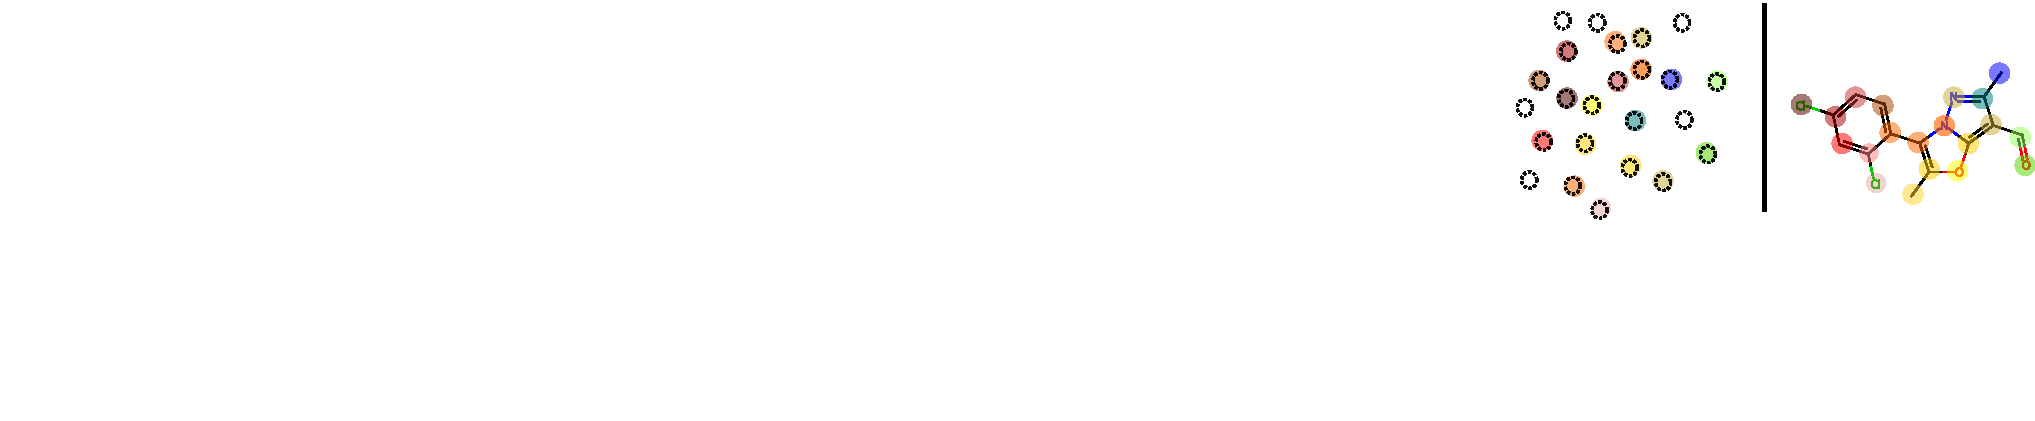
\includegraphics[width=10cm,height=7cm,keepaspectratio]{fig/product.pdf}};
% Scope for drawing on image
% Labels
\node[text width=10cm, align=center] at (-20,4) {Target (reactants)};
\node[text width=10cm, align=center] at (8,4) {Input (product)};
\node[text width=1cm, align=center] at (8.5,-4) {$\Y$};
\node[text width=1cm, align=center] at (3.5,-4) {$\X_T$};
\node[text width=1cm, align=center] at (-8,-4) {$\X_t$};
\node[text width=1cm, align=center] at (-20,-4) {$\X_0$};
\node (c0) at (-2.6,0) {};
\node[text width=1cm, align=center] at ($(c0) + (-1,2)$) {\scalebox{.7}{$q(\X_t\!\mid\!\X_{t-1})$}};
\node[text width=1cm, align=center] at ($(c0) + (-1,-2)$) {\scalebox{.7}{$p_\theta(\X_{t-1}\!\mid\!\X_t,\!\Y)$}};
\node[text width=1cm, align=center] at ($(c0) + (1,-6)$) {\scalebox{.7}{$=\sum_{\X_0}q(\X_0\!\mid\!\X_T,\!\X_0)p_\theta(\X_{0}\!\mid\!\X_{T},\!\Y,\!\P^{\Y\to\X})$}};
\node (c0) at (-13.5,0) {};
\node[text width=1cm, align=center][text width=1cm, align=center][text width=1cm, align=center] at ($(c0) + (-2,2)$) {\scalebox{.7}{$q(\X_{t+1}\!\mid\!\X_{t})$}};
\node[text width=1cm, align=center] at ($(c0) + (-2,.-2)$) {\scalebox{.7}{$p_\theta(\X_{t}\!\mid\!\X_{t+1},\!\Y)$}};
\end{tikzpicture}

\end{document}